\documentclass[11pt]{report}
\usepackage{amssymb,amsmath}
\usepackage[utf8]{inputenc}

\usepackage[T1]{fontenc}

\usepackage[francais]{babel}
\usepackage{graphicx}
\usepackage[top=2cm, bottom=2cm, left=2cm, right=2cm]{geometry} %pour modifier les marges
\usepackage{setspace} % pour modifier les interlignes
\usepackage{array}


\renewcommand{\thesection}{\Roman{section}}
\newcommand{\deriv}{\mathrm{d}}


%création de la page de garde
\title{{\huge Signal et Filtrage - Corrections des exercices}} 
\author{Alexandre Boyer, Pascal Acco, Léa Cot, Etienne Sicard}
\date{Septembre 2019}

\begin{document}
	\maketitle
	
	\textbf{Signal \& Filtrage}
	
	\textbf{}\\
	
	2 IMACS
	
	2019 - 2020
	
	alexandre.boyer@insa-toulouse.fr	
	page Moodle
	
	
\chapter{L'étude de la réponse des systèmes linéaires à temps invariant}

	\subsubsection{Exercice 1} 
	Soient les systèmes dont le comportement temporel est défini par les équations suivantes. Indiquez si ces systèmes sont linéaires, à temps invariant et causaux ?
	
	a. $y(t) = x(t)+4\frac{dy}{dt}$ 
	
	b. $y(t) = 2x(t)+2$ 
	
	c. $y(t)=e^{-t}x(t-2)^{2}$
	
	d. $y(t)=\frac{dx}{dt}+x(t+2)$
	
	\vspace{1\baselineskip}
	

	
	\textbf{\underline{Correction exercice 1}}\\
	a. On vérifie facilement que le système est :
	 \begin{itemize}
	 	\item linéaire (soit $x_{1}(t) $ et $x_{2}(t)$ les solutions de l'équation pour $y_{1}(t)$ et $y_{2}(t)$. $x(t)=ax_{1}(t)+bx_{2}(t)$ ne peut être la solution que de $y(t)=ay_{1}(t)+by_{2}(t)$).
	 	\item à temps invariant (les paramètres de l'équation sont invariants dans le temps)
	 	\item causal (la sortie ne dépend pas des états futurs de l'entrée et de la sortie).
	 \end{itemize}
 	\vspace{0.5\baselineskip}
 	b. Le système est causal et à temps invariant, mais n'est pas linéaire. Soit  $x_{1}(t) $ et $x_{2}(t)$ les solutions de l'équation pour $y_{1}(t)$ et $y_{2}(t)$. $x(t)= ax_{1}(t)+bx_{2}(t)$ est la solution de $y(t)=2ax_{1}(t)+2+2bx_{2}(t)+2 \neq ay_{1}(t)+by_{2}(t)=2ax_{1}(t)+2a+2bx_{2}(t)+2b$
 	
 	\vspace{0.5\baselineskip}
 	c. Le système n'est ni linéaire ( $x(t)= ax_{1}(t)+bx_{2}(t)$ est la solution de $e^{-t}(ax_{1}(t-2)+bx_{2}(t-2))^{2} \neq ae^{-t}x_{1}(t-2)^{2}+be^{-t}x_{2}(t-2)^{2}$), ni à temps invariant (le coefficient devant $x^{2}$ dépend du temps). Le système est causal (la sortie à l'instant t dépend de l'entrée donnée à un instant passé (t-2)).
 	
 	\vspace{0.5\baselineskip}
 	d. Le système est linéaire et à temps invariant, mais n'est pas causal puisque la sortie à un instant t dépend de l'entrée à un instant futur (t+2).
 	
 	\vspace{1\baselineskip}
 	
 	
 	\subsubsection{Exercice 2} 
 	1. On trace les réponses de deux systèmes LTI. Proposez une expression mathématique décrivant ces réponses.
 	\begin{figure}[h!]
 		\centering
 		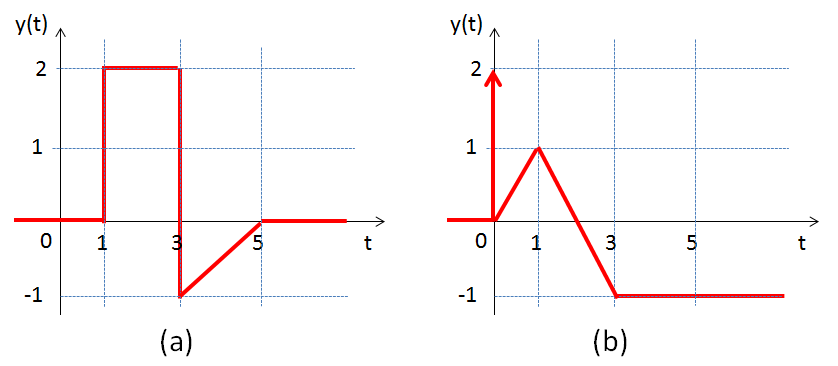
\includegraphics[scale=0.5]{images/Exo_2_2.jpg} 
 	\end{figure} \\
 
 	\vspace{0.5\baselineskip}
 	
 	2. Réécrivez sous la forme d'une fonction à valeurs réelles les fonctions suivantes et esquissez leur forme temporelle (pour t >0) :
 	
 	a. $x(t) = (1+j)e^{j\cdot 10t}$ 
 	
 	b. $y(t) = e^{(-2+j)t}\cdot u(t-2)$ 
 	
 	c. $z(t) = e^{(-1+2j)t}+e^{(-1-2j)t}$
 	
 	\vspace{1\baselineskip}	
 	
 	\subsubsection{Exercice 3 - Réponse indicielle d'un circuit RC}
 	
 	On reprend le circuit RC dont on a étudié la réponse dans la partie VI.3. On considère deux cas : celui où le condensateur est déchargé initialement, puis celui où il est chargé. 
 	
 	a. Calculez la réponse naturelle du circuit lorsque le condensateur est initialement chargé.
 	
 	b. En déduire la réponse impulsionnelle du circuit.
 	
 	c. Calculez la réponse lorsque le circuit est soumis à un échelon de Heaviside d'amplitude E, dans les deux cas (charge initiale absente ou présente).
 	
 	d. En déduire la réponse indicielle du circuit.
 	 
 	\vspace{1\baselineskip}
 	
 	\subsubsection{Exercice 4}
 	
 	On considère les deux circuits électriques ci-dessous. Pour le circuit (a), la tension initiale (t=0) aux bornes du condensateur C est notée $U_{C0}$. Pour le circuit (b), un courant noté $I_L0$ traverse la bobine L. La sortie de ces deux circuits est la tension $U_{S}$.
 	
 	\begin{figure}[h!]
 		\centering
 		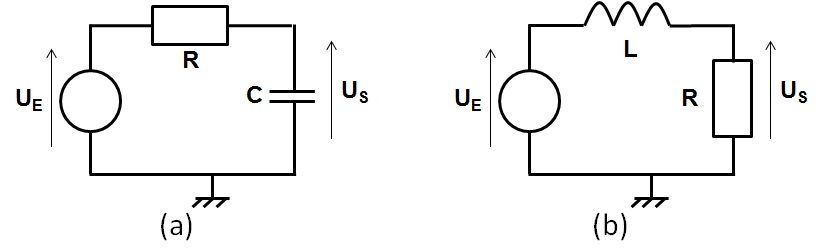
\includegraphics[scale=0.5]{images/Exo_2_4.jpg} 
 	\end{figure} 
 	
 	a. Déterminez les fréquences et les réponses naturelles de ces deux circuits. Quel est l'ordre de ces deux systèmes ? 
 	
 	b. On excite ces deux systèmes à l'aide d'un échelon de Heaviside d'amplitude notée E. Déterminez la réponse indicielle de ces deux circuits. 
 	
 	c. Déterminez les fonctions de transfert de ces deux circuits.
 	
 	\vspace{1\baselineskip}
 	
 	\subsubsection{Exercice 5 - Fonction de transfert d'un circuit résonant}
 	
 	On reprendre le circuit RLC présenté dans la partie IV.4. Celui-ci est excité par un générateur de courant I, comme le montre la figure ci-dessous. On s'intéresse à la tension U aux bornes de ce circuit RLC. 
 	 	
 	\begin{figure}[h!]
 		\centering
 		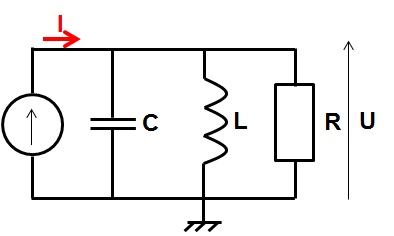
\includegraphics[scale=0.5]{images/Exo_2_5.jpg} 
 	\end{figure} 
 
 	a. Déterminez la fonction de transfert de ce circuit. 
 	
 	b. Précisez l'unité de la fonction de transfert. 
 	
 	c. Dans le cas où l'on considère une excitation cosinusoïdale du circuit, y a t-il une fréquence particulière où la réponse présente un maximum ? Si oui, laquelle ? Donnez l'expression de la réponse temporelle du circuit en régime permanent.
 	
 	\vspace{1\baselineskip}
 	
 	\subsubsection{Exercice 6}
 	
 	On considère le système dont le fonctionnement est décrit par le schéma-bloc ci-dessous. Celui-ci transforme un signal d'entrée e(t) et délivre en sortie un signal s(t). 
 	
 	\begin{figure}[h!]
 		\centering
 		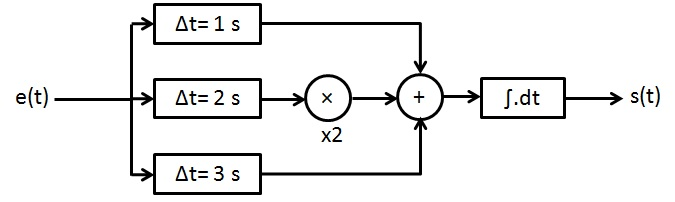
\includegraphics[scale=0.5]{images/Exo_2_6.jpg} 
 	\end{figure}
 
 	a. Le système est-il linéaire, à temps invariant, causal ?
 	
 	b. Déterminez l'expression de la réponse impulsionnelle h(t) du système. Esquissez l'allure temporelle de la réponse impulsionnelle. 
 	
 	c. Déterminez l'expression de la fonction de transfert H(p) du système. Précisez les pôles et les zéros de la fonction de transfert. Que concluez-vous sur sa stabilité ?
 
 	\vspace{1\baselineskip}
 	
 		\textbf{\underline{Correction exercice 6}}\\
 	a. Le système transforme le signal d'entrée à partir de trois opérations de base : retard, multiplication par une constante et intégration temporelle. Il s'agit d'opérations purement linéaires. Le fonctionnement du système est indépendant du temps. Il s'agit donc d'un système LTI. De plus, il est causal puisque la sortie ne dépend que des états passés du signal d'entrée.
 	
 	b. On considère une entrée égale à une impulsion de Dirac : $e(t) = \delta(t)$.	Avant l'intégrateur, le signal résultant s'écrit : $e(t-1)+2e(t-2)+e(t-3)=\delta(t-1)+2\delta(t-2)+\delta(t-3)$. L'impulsion de Dirac résultant de la dérivée de l'échelon de Heaviside, après intégration, la sortie du système est donnée par : $s(t) = h(t) = u(t-1)+2u(t-2)+u(t-3)$.
 	
	
	\newpage
	
	\chapter{Transformée de Laplace}
	
	
	\subsubsection{Exercice 1}
	
	Déterminez les transformées de Laplace des fonctions suivantes :
	
	a. $x(t)=e^{-2t}u(t-1)$
	
	b. $y(t)=e^{-2(t-1)}u(t-1)$
	
	c. $z(t) = \sqrt{2}cos(t+\frac{\pi}{4})$
	
	\begin{figure}[h!]
		\centering
		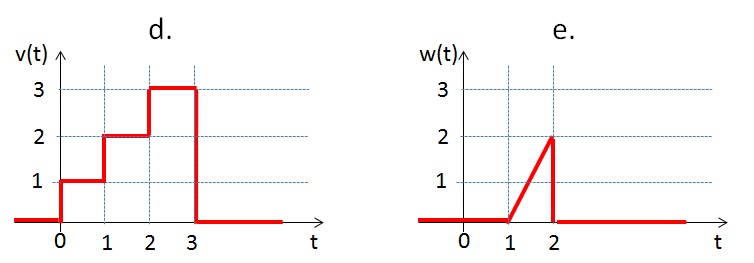
\includegraphics[scale=0.5]{images/Exo_2_1_a.jpg} 
	\end{figure} 

	\begin{figure}[h!]
		\centering
		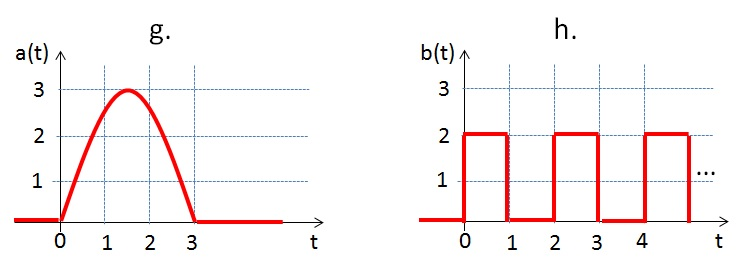
\includegraphics[scale=0.5]{images/Exo_2_1_b.jpg} 
	\end{figure}
	
	
	
	\vspace{1\baselineskip}
	
	\textbf{\underline{Correction exercice 1}}\\
	a. Attention à ne pas utiliser le théorème du retard trop hâtivement (seul l'échelon de Heaviside est retardé) !
	
	$X(p) = \int_{0}^{+\infty} e^{-2t}u(t-1)e^{-pt}dt=\int_{1}^{+\infty} e^{-(p+2)t}dt=\frac{e^{-(p+2)}}{p+2}$
	
	\vspace{0.5\baselineskip}
	
	b. Théorème du retard : $Y(p) = \frac{e^{-p}}{p+2}$
	
	\vspace{0.5\baselineskip}
	
	c. $z(t) = \sqrt{2}(cos(t)cos(\frac{\pi}{4})-sin(t)sin(\frac{\pi}{4}))=cos(t)-sin(t)$
	
	$Z(p) = \frac{p}{p^{2}+1}-\frac{1}{p^{2}+1}=\frac{p-1}{p^{2}+1}$
	
	\vspace{0.5\baselineskip}
	
	d. $v(t) = u(t)+u(t-1)+u(t-2)-3u(t-3)~\Rightarrow~V(p)=\frac{1+e^{-p}+e^{-2p}-3e^{-3p}}{p}$ 
	
	\vspace{0.5\baselineskip}
	
	e. $w(t) = 2(t-1)u(t-1)-2(t-2)u(t-2)-2u(t-2)~\Rightarrow~W(p)=\frac{2e^{-p}}{p^{2}}(1-e^{-p}-pe^{-p})$ 
	
	\vspace{0.5\baselineskip}
	
	g. $a(t)=3sin(\frac{\pi}{3}t)u(t)+3sin(\frac{\pi}{3}(t-3))u(t-3)~\Rightarrow~A(p)=\frac{\pi(1+e^{-3p})}{p^{2}+(\frac{\pi}{3})^{2}}$
	
	\vspace{0.5\baselineskip}
	
	h. Il s'agit d'une fonction périodique. En déterminant la transformée de Laplace de la fonction génératrice $B_{0}(p)$, on pourra déterminer ensuite celle de la fonction périodique $B(p)$.
	
	$b_{0}(t)=2u(t)-2u(t-1)~\Rightarrow~B_{0}(p)=2\frac{1-e^{-p}}{p}$
	
	La périodicité d'une fonction de période T se traduit, dans le domaine de Laplace par une multiplication par le terme : $\frac{1}{1-e^{pT}}$. La transformée de Laplace de la fonction b(t), de période T = 2, s'écrit donc : $B(p) =2\frac{1-e^{-p}}{p(1-e^{2p})} $.
	
	\vspace{0.5\baselineskip}
	
	
	\subsubsection{Exercice 2}
	
	Déterminez les expressions temporelles des fonctions suivantes :
	
	a. $X(p)=\frac{p-4}{p^{2}+16}$ 
	
	b. $Y(p) = \frac{p^{2}+3p+3-\frac{6}{p}}{p^{2}}$ 
	
	c. $Z(p) = \frac{p^{2}+4p+4}{p^{2}+2p+2}$
	
	d. $W(p) = \frac{p-1+e^{-p}}{p^{2}(1-e^{-p})}$. Tracez cette fonction.
	
	
	\vspace{1\baselineskip}
	
	\textbf{\underline{Correction exercice 2}}\\
	
	a. $x(t)=[cos(4t)-sin(4t)]u(t)$
	
	b. $Y(p)=1+\frac{3}{p}+\frac{3}{p^{2}}-\frac{6}{p^{3}} ~~\Longrightarrow~ y(t)=\delta(t)+3u(t)+3t\cdot u(t)-6t^{2}\cdot u(t)$
	
	c. $Z(p)=1+\frac{2p+2}{p^{2}+2p+2}~~\Longrightarrow~z(t)=\delta(t)+2e^{-t}cos(t)u(t)$
	
	d. Laissons d'abord de côté le terme $\frac{1}{1-e^{-p}}$ car il indique une périodicité de période T=1. Soit la fonction $W_{1}(p)= \frac{p-1+e^{-p}}{p^{2}}=\frac{1}{p}-\frac{1}{p^{2}}+\frac{e^{-p}}{p^{2}}$. On en déduit $w_{1}(t)=u(t)-tu(t)+(t-1)u(t)$ (pour le dernier terme, utilisation du théorème du retard). La fonction $w(t) =w_{1}(t-kT)$, avec k > 0. Cela correspond à une fonction périodique en dent de scie.
	
	
	\vspace{1\baselineskip}
	
	\subsubsection{Exercice 3}
	
	Résoudre les équation différentielles suivantes :
	
	a. $x"+2x'+x=e^{-t}u(t)$, avec x(0) = 0 et x'(0) = 0. 
	
	b. $x"+6x'+8x=\delta(t)$ avec x(0)=1 et x'(0)=3. 
	
	\vspace{1\baselineskip}
	
	\textbf{\underline{Correction exercice 3}}\\
	
	a. $p^{2}X(p)+2pX(p)+X(p)=\frac{1}{p+1}~\Rightarrow X(p)=\frac{1}{(p+1)^{3}}$. En considérant le théorème de translation de p, en posant P=p+1 : $X(P)=\frac{1}{P^{3}}$, soit $X(t)=t^{2}u(t)$, qui devient après changement de variable : $x(t)=e^{-t}t^{2}u(t)$.
	
	b. $X(p)=\frac{p+10}{(p+2)(p+4)} = \frac{4}{p+2}-\frac{3}{p+4}$, d'où $x(t) = (4e^{-2t}-3e^{-4t})u(t)$.
	
	\vspace{1\baselineskip}
	
	
	\subsubsection{Exercice 4}
	
	On reprend l'exercice 6 du chapitre 2.
	
	
	\begin{figure}[h!]
		\centering
		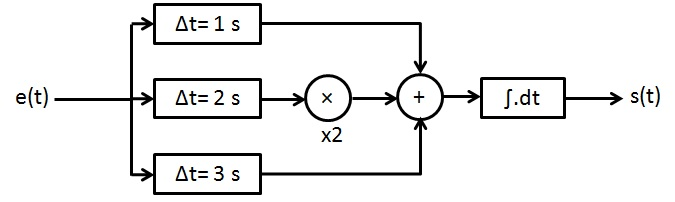
\includegraphics[scale=0.5]{images/Exo_2_6.jpg} 
	\end{figure}
	
	a. Ecrivez la fonction de transfert du système dans le domaine de Laplace.
	
	b. Calculez la réponse indicielle du système. On supposera que les conditions initiales de tous les nœuds internes du système sont nulles. 
	
	
	\vspace{1\baselineskip}
	
		
	\subsubsection{Exercice 5}
	
	On considère un circuit électrique, dont le courant i(t) est donné par l'équation ci-dessous.
	\begin{equation*}
		e(t)=\frac{d^{2}i}{dt^{2}}+7\frac{di}{dt}+10i(t)
	\end{equation*}
	On considère l'excitation suivante $e(t)=6e^{-3t}u(t)$. Les conditions initiales du circuit sont : $i(0) = 3~A$ et $\frac{di}{dt}(0)=3~A/s$.
	
	
	a. Etablir l'expression du courant dans le domaine de Laplace.
	
	b. En déduire l'expression temporelle du courant i(t).
	
	c. Vérifiez, en utilisant les expressions du courant dans le domaine de Laplace, puis dans le domaine temporel, que la condition initiale du courant est respectée. Déterminez ensuite les conditions finales.
	
	\vspace{1\baselineskip}
	
	\textbf{\underline{Correction exercice 5}}\\
	a. A partir de l'équation différentielle et des conditions initiales, la transformée de Laplace est la suivante :
	
	\begin{equation*}
		p^{2}I(p)-pi(0)-i(0)+7pI(p)-7i(0)+10I(p)=\frac{6}{p+3}
	\end{equation*}
	On transforme ensuite cette relation pour exprimer I(p) sous la forme d'une somme d'éléments dont nous disposons l'expression temporelle (par exemple, fonction rationnelle).
	\begin{equation*}
	I(p)\cdot (p^{2}+7p+10)=\frac{6}{p+3}+3(p+8)
	\end{equation*}
	\begin{equation*}
	I(p)\cdot (p+2)(p+5)=\frac{3(p^{2}+11p+26)}{p+3}
	\end{equation*}
	\begin{equation*}
	I(p)=\frac{3(p^{2}+11p+26)}{(p+3)(p+2)(p+5)}
	\end{equation*}
	En utilisant la méthode du cache, on décompose en pôles et résidus l'expression précédente.
	\begin{equation*}
		I(p)=\frac{A}{p+2}+\frac{B}{p+3}+\frac{C}{p+5}
	\end{equation*}
	\begin{equation*}
		(p+2)I(p)=\frac{3(p^{2}+11p+26)}{(p+3)(p+5)}=A+\frac{B(p+2)}{p+3}+\frac{C(p+2)}{p+5}~\rightarrow~p=-2~:~A=\frac{3((-2)^{2}+11\cdot (-2)+26)}{(-2+3)(-2+5)}=8
	\end{equation*}
	\begin{equation*}
	(p+3)I(p)=\frac{3(p^{2}+11p+26)}{(p+2)(p+5)}=\frac{A(p+3)}{p+2}+B+\frac{C(p+3)}{p+5}~\rightarrow~p=-3~:~B=\frac{3((-3)^{2}+11\cdot (-3)+26)}{(-3+2)(-3+5)}=-3
	\end{equation*}
	\begin{equation*}
	(p+5)I(p)=\frac{3(p^{2}+11p+26)}{(p+2)(p+3)}=\frac{A(p+5)}{p+2}+\frac{B(p+5)}{p+3}+C~\rightarrow~p=-5~:~C=\frac{3((-5)^{2}+11\cdot (-5)+26)}{(-5+2)(-5+3)}=-2
	\end{equation*}
	L'expression du courant dans le domaine de Laplace peut s'écrire de la manière suivante :
	\begin{equation*}
		I(p)=\frac{8}{p+2}-\frac{3}{p+3}-\frac{2}{p+5}
	\end{equation*}
	
	\vspace{0.5\baselineskip}
	
	b. A partir de l'expression précédente, on en déduit directement la forme temporelle du courant à l'aide de la table des transformées de Laplace inverse usuelles.
	\begin{equation*}
	i(t)=(8e^{-2t}-3e^{-3t}-2e^{-5t})u(t)
	\end{equation*}
	
	\vspace{0.5\baselineskip}
	
	c. Condition initiale du courant : d'après les propriétés de la transformée de Laplace, on sait que :
	\begin{equation*}
		\lim_{t\rightarrow0^{+}} i(t)=\lim_{p \to +\infty} pI(p)
	\end{equation*}
	On vérifie cette égalité en retrouvant la valeur de la condition initiale du courant.
	\begin{equation*}
		\lim_{t\rightarrow0^{+}} i(t)=\lim_{t\rightarrow0^{+}}(8e^{-2t}-3e^{-3t}-2e^{-5t})u(t)=8-3-2=3~A
	\end{equation*}
	\begin{equation*}
		\lim_{p \to +\infty} pI(p)=	\lim_{p \to +\infty} \frac{8p}{p+2}-\frac{3p}{p+3}-\frac{2p}{p+5}=8-3-2=3~A
	\end{equation*}
	
	Condition finale du courant : d'après les propriétés de la transformée de Laplace, on doit vérifier que :
	\begin{equation*}
	\lim_{t \to +\infty} i(t)=\lim_{p \to 0} pI(p)
	\end{equation*}
	
	On détermine ainsi la valeur finale du courant.
	\begin{equation*}
	\lim_{t \to +\infty} i(t)=\lim_{t \to +\infty}(8e^{-2t}-3e^{-3t}-2e^{-5t})u(t)=0~A
	\end{equation*}
	\begin{equation*}
	\lim_{p \to 0} pI(p)=	\lim_{p \to 0} \frac{8p}{p+2}-\frac{3p}{p+3}-\frac{2p}{p+5}=0~A
	\end{equation*}
	
	\vspace{1\baselineskip}
	
	
	\subsubsection{Exercice 6 - Réponse d'un moteur à courant continu à aimants permanents}

	Le fonctionnement d'un moteur est gouverné par un modèle électromécanique, se présentant sous la forme de plusieurs équations différentielles reliant grandeurs électriques et mécaniques. Dans cet exercice, nous allons étudier le modèle simplifié d'un moteur à courant continu à aimants permanents. La figure ci-dessous présente le modèle électrique équivalent de l'induit. Celui-ci est modélisé par un circuit RL et est excité par une tension de commande notée $U_{C}$. Lorsque le moteur tourne, une force contre électromotrice (fcem) E est induite, qui est proportionnelle à la vitesse angulaire du moteur $\Omega$. 
	\begin{figure}[h!]
		\centering
		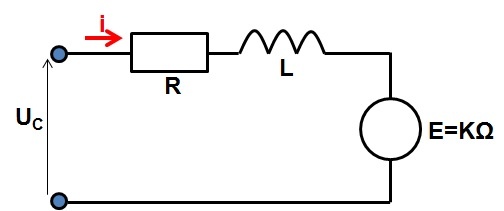
\includegraphics[scale=0.5]{images/Exo3_moteur.jpg} 
	\end{figure}	
	Le courant i circulant dans l'induit produit un couple moteur $C_{m}$, selon la même constante de proportionnalité K que celle liant la fcem et la vitesse de rotation du moteur. A ce couple moteur s'opposent plusieurs sources de couples résistants $C_{R}$ :
	\begin{itemize}
		\item l'inertie du moteur, donnée par le moment d'inertie J
		\item les frottements visqueux, caractérisés par le coefficient de frottement visqueux f
	\end{itemize}
	L'équation mécanique du moteur s'écrit alors :
	\begin{equation*}
		C_{m} = C_{R} = J\frac{d\Omega}{dt}+f\Omega
	\end{equation*}	
	Nous cherchons à déterminer la vitesse de rotation du moteur en fonction de l'excitation appliquée.
	Dans cet exercice, on considèrera les valeurs suivantes : r=0.2 $\Omega$, L = 0.2 mH, K = 0.057 N.m/A, J = $650.10^{-7}~kg.m^{2}$, f = $2.3.10^{-5}~N.m/rad.s^{-1}$. On suppose que le moteur est initialement à l'arrêt.
	
	a. Etablir l'équation différentielle reliant la vitesse de rotation et l'excitation $U_{C}$ du moteur.
	
	b. Déterminez la fonction de transfert du moteur dans le domaine de Laplace. Exprimez-la sous la forme $\frac{G}{p^{2}+2\alpha p+\omega_{0}^{2}}$.
	
	c. Calculez les pôles du système. Est-il stable ?
	
	d. En t = 0, on applique une commande de type échelon unitaire d'amplitude $Uc_{0}$ = 10 V. Déterminez l'expression du profil temporel de la vitesse angulaire.
	
	e. Esquissez le profil temporel de la vitesse angulaire. En régime permanent, quelle est la valeur de la vitesse ? 
	
	
	\newpage
	
	\chapter{Filtrage}
	
	\subsubsection{Exercice 1}
	Soit les fonctions de transfert suivantes. Esquissez le diagramme de Bode (asymptotique). 
	
	\subsubsection{Exercice 2}
	Soit les 3 tracés asymptotiques dans le diagramme de Bode présentés ci-dessous. Proposez les fonctions de transfert possibles pour chacune d'elles. 
	
	
	\subsubsection{Exercice 3}
	On considère le filtre ci-dessous (CRRC). On utilisera les valeurs suivantes
	
	1. Déterminez l'expression littérale de la fonction de transfert. Précisez les pôles et les zéros du filtre.
	
	2. On se place en régime harmonique. Quelles sont les fréquences de coupure ?
	
	3. Tracez le diagramme de Bode de ce filtre. Quelle est la nature du filtre ? Précisez son ordre.
	
	4. Parmi les trois signaux suivants (harmoniques), lesquelles sont transmis en sortie de filtre ?
	
	\subsubsection{Exercice 4}
	On dispose d'un filtre dont la fonction de transfert est donnée par : (filtre passe-bas)
	On l'attaque avec les signaux suivants : impulsion de largeur tau, puis une impulsion avec une montée Tr.
	
	1. Tracez la réponse fréquentielle du filtre dans le diagramme de Bode. Quelle est la nature du filtre ?
	
	2. Pour les deux signaux d'excitation, déterminez l'expression théorique de la réponse du filtre.
	
	3. Déterminez l'amplitude du signal de sortie pour tau = xx puis yy. Même chos avec Tr = xx et yy. Conclure sur l'effet du filtre sur des signaux impulsionnels.
	
	On peut faire un exo similaire avec un filtre passe-haut.
	
	
	\subsubsection{Exercice 5 - Calcul d'une impédance}
	
	Ce serait bien de faire un exo de filtrage avec comme entrée I et comme sortie V, ce qui donnerait une unité au filtre : impédance.
	
	
	\subsubsection{Exercice 5 - Mise en cascade de filtres}
	On considère le filtre RC ci-dessous.
	
	\begin{figure}[h!]
		\centering
		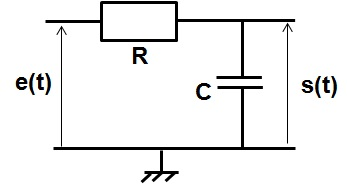
\includegraphics[scale=0.5]{images/Filtre_RC_passe_bas.jpg} 
	\end{figure}

	1. Calculez la fonction de transfert de ce filtre H(f).
	
	2. Précisez sa nature, sa fréquence de coupure, son ordre.
	
	3. On cascade deux filtres de ce type. Calculez sa fonction de transfert $H_{2}(f)$.
	
	4. Vérifie t-on $H_{2}(f)=H(f)^{2}$ ? Pourquoi ?
	
	\vspace{1\baselineskip}
	
	\textbf{\underline{Correction exercice 5}}\\
	1. $H(f)=\frac{1}{RC}\frac{1}{j2\pi f+\frac{1}{RC}}$
	
	2. Filtre passe-bas d'ordre 1. La fréquence de coupure $f_{c}=\frac{1}{2^pi RC}$
	
	3. On peut montrer que :
	\begin{equation*}
	\frac{s_{1}}{e}(p)=\frac{Z_{eq}}{R+Z_{eq}}~avec~Z_{eq}=\frac{1+RCp}{Cp(2+RCp)}
	\end{equation*}
	\begin{equation*}
	\frac{s_{1}}{e}(p)=\frac{1}{RC}\frac{p+\frac{1}{RC}}{p^{2}+\frac{3}{RC}p+\frac{1}{RC}^{2}}
	\end{equation*}
	
	\begin{figure}[h!]
		\centering
		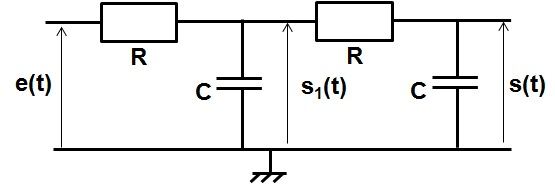
\includegraphics[scale=0.5]{images/Cascade_filtre_RC_passe_bas.jpg} 
	\end{figure}

	\begin{equation*}
	\frac{s}{s_{1}}(p)=\frac{1}{RC}\frac{1}{p+\frac{1}{RC}}
	\end{equation*}
	On en déduit l'expression de la fonction de transfert :
	\begin{equation*}
	H_{2}(p)=\frac{s}{s_{1}}(p)\cdot \frac{s_{1}}{e}(p)=\frac{1}{RC}^{2}\frac{1}{p^{2}+\frac{3}{RC}p+\frac{1}{RC}^{2}}
	\end{equation*} 
	\begin{equation*}
	\frac{s_{1}}{e}(p)=\frac{1}{RC}^{2}\frac{1}{(j2\pi f)^{2}+\frac{3}{RC}(j2\pi f)+\frac{1}{RC}^{2}}
	\end{equation*}
	On reconnait la fonction de transfert d'un filtre passe bas d'ordre 2.
	
	4. En appliquant la formule de mise en cascade des fonctions de transfert des deux cellules RC, on trouve :
	\begin{equation*}
	H(f)H(f)==\frac{1}{RC}^{2}\frac{1}{(j2\pi f)^{2}+\frac{1}{RC}(j2\pi f)+\frac{1}{RC}^{2}} \neq H_{2}(f)
	\end{equation*}
	La mise en cascade des fonctions de transfert suppose que la deuxième cellule n'influe pas sur la tension en sortie de la première cellule ($s_{1}$), ce qui n'est pas le cas. La tension mesurée $s_{1}$ dépend de l'impédance connectée en ce nœud (impédance $Z_{eq}$). La figure ci-dessous compare les fonctions de transfert $H_{2}(f)$ et $H(f)H(f)$
	
	\begin{figure}[h!]
		\centering
		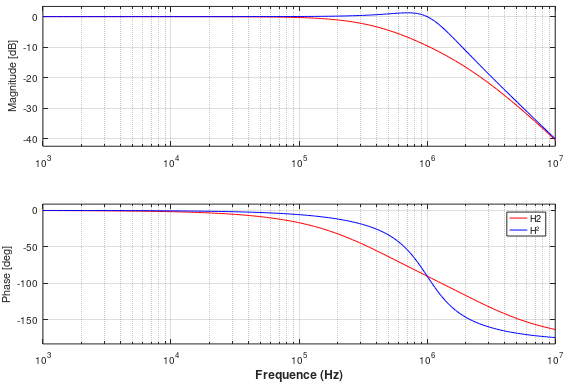
\includegraphics[scale=0.6]{images/Effet_cascade_filtre_RC.png} 
	\end{figure}
	
	 
	
	
	
	
	
	
	
	\vspace{1\baselineskip}
	
	
	\newpage
	
	\chapter{Analyse des systèmes et des signaux dans le domaine temporel}
	
	\subsubsection{Exercice 1}
	
	Déduire les réponses impulsionnelles de système à partir de transformée de Fourier, Laplace et de réponse indicielle
		
	\subsubsection{Exercice 2}
	
	On considère les fonctions h(t) et x(t) dont le profil est représenté ci-dessous.
	\begin{figure}[h!]
		\centering
		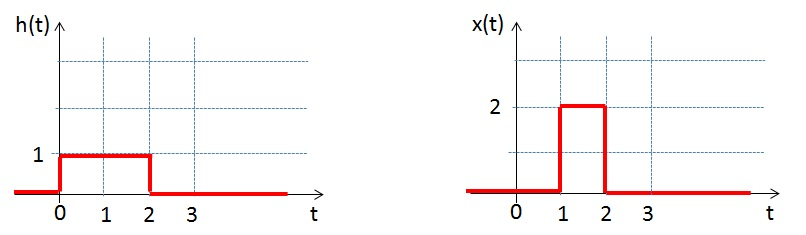
\includegraphics[scale=0.5]{images/Courbes_TD_Convolution_2.jpg} 
	\end{figure}
	
	1. Proposez une expression mathématique pour ces deux fonctions.
	
	2. On note y(t) le résultat du produit de convolution de x(t) et h(t). Déterminez l'expression de y(t) en calculant directement le produit de convolution. Tracez l'allure de cette fonction.
	
	3. En utilisant la transformée de Laplace, vérifiez la validité du résultat précédent.
	
	4. Même chose en utilisant la transformée de Fourier.
	
	\vspace{1\baselineskip}
	
	\textbf{\underline{Correction exercice 2}}\\
	
	1. $h(t)=u(t)-u(t-2)$ et $x(t)=2(u(t-1)-u(t-2))$.
	
	2. Graphiquement, on peut déduire l'allure de $y(t)=\int_{-\infty}^{+\infty}h(\tau)x(t-\tau)d\tau$. En traçant $h(\tau)$ et $x(t-\tau)$, on distingue 5 intervalles différents :
	\begin{itemize}
		\item si t < 1 ou t > 4, alors $h(\tau)$ et $x(t-\tau)$ ne se recouvrent jamais, donc l'intégrale $y(t)=\int_{-\infty}^{+\infty}h(\tau)x(t-\tau)d\tau = 0$.
		\item si $1 \leq t<2$, alors l'aire sous l'intersection des courbes $h(\tau)$ et $x(t-\tau)$ croit linéairement quand t augmente.
		\item si $2 \leq t < 3$, alors l'aire sous l'intersection des courbes $h(\tau)$ et $x(t-\tau)$ est maximale, constante et égale à 2.
		\item si $3 \leq t < 4$,  alors l'aire sous l'intersection des courbes $h(\tau)$ et $x(t-\tau)$ décroit linéairement quand t augmente.
	\end{itemize}
	
	L'allure de y(t) est présentée ci-dessous. On peut en déduire l'expression suivante :
	\begin{equation*}
	y(t)=2[(t-1)u(t-1)-(t-2)u(t-2)-(t-3)u(t-3)+(t-4)u(t-4)]
	\end{equation*}
	\begin{figure}[h!]
		\centering
		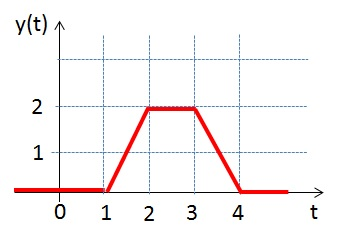
\includegraphics[scale=0.6]{images/Courbes_TD_Convolution_2_Solution.jpg} 
	\end{figure}

	Cette expression peut aussi être déduite en résolvant directement l'intégrale du produit de convolution :
	\begin{equation*}
	y(t)=2\int_{-\infty}^{+\infty}(u(\tau)-u(\tau-2))\cdot (u(t-(\tau-1))-u(t-(\tau-2)))d\tau
	\end{equation*}
	\begin{equation*}
	y(t)=2\int_{-\infty}^{+\infty}[u(\tau)u(t-(\tau-1))-u(\tau)u(t-(\tau-2))-u(\tau-2)u(t-(\tau-1))+u(\tau-2)u(t-(\tau-2))]d\tau
	\end{equation*}
	On distingue quatre termes dans l'intégrale, qui peuvent être calculés individuellement :
	\begin{itemize}
		\item $\int_{-\infty}^{+\infty}u(\tau)u(t-(\tau-1))d\tau=(t-1)u(t-1)$
		\item $\int_{-\infty}^{+\infty}u(\tau)u(t-(\tau-2))d\tau=(t-2)u(t-2)$
		\item $\int_{-\infty}^{+\infty}u(\tau-2)u(t-(\tau-1))d\tau=(t-3)u(t-3)$
		\item $\int_{-\infty}^{+\infty}u(\tau-2)u(t-(\tau-2))d\tau=(t-4)u(t-4)$
	\end{itemize}
	En addition ces différentes contributions, on retrouve le résultat précédent :
	$y(t)=2[(t-1)u(t-1)-(t-2)u(t-2)-(t-3)u(t-3)+(t-4)u(t-4)]$.
	
	\vspace{0.5\baselineskip}
	
	3. La validité du résultat précédent peut facilement être vérifiée en utilisant la transformée de Laplace. En effet, le produit de convolution se transforme en un simple produit dans le domaine des fréquences complexes.
	Les transformées de Laplace de h(t) et x(t) peuvent facilement être dérivées à partir de la table des transformées de Laplace courantes : $H(p) = \frac{1}{p}-\frac{e^{-2p}}{p}$ et $X(p)=\frac{2e^{-p}}{p}-\frac{2e^{-2p}}{p}$. La transformée de Laplace Y(p) est déterminée en multipliant les deux termes précédents :
	\begin{equation*}
	Y(p)=(\frac{1}{p}-\frac{e^{-2p}}{p})\cdot(\frac{2e^{-p}}{p}-\frac{2e^{-2p}}{p})=\frac{2e^{-p}}{p^{2}}-\frac{2e^{-2p}}{p^{2}}-\frac{2e^{-3p}}{p^{2}}+\frac{2e^{-4p}}{p^{2}}
	\end{equation*}
	En utilisant la transformée de Laplace inverse, on retrouve la même expression pour y(t) que dans la question précédente.
	
		$y(t)=\mathcal{L}^{-1}[Y(p)]=2[(t-1)u(t-1)-(t-2)u(t-2)-(t-3)u(t-3)+(t-4)u(t-4)]$
	
	\vspace{0.5\baselineskip}
	
	4. Le même genre de vérification peut être réalisée en utilisant la transformée de Fourier. Les fonctions h(t) et x(t) sont deux fonctions portes de largeur T=2 et T=1 respectivement. Elles sont centrées sur 1 et 1.5 respectivement. Leurs transformées de Fourier sont données par :
	\begin{equation*}
	H(f)=2sinc(2f)e^{j2\pi f}=2\frac{sin(2\pi f)}{2\pi f}e^{j2\pi f}
	\end{equation*}
	\begin{equation*}
	X(f)=2sinc(f)e^{j2\pi f\cdot \frac{3}{2}}=2\frac{sin(\pi f)}{\pi f}e^{j2\pi f\cdot \frac{3}{2}}
	\end{equation*}
	La transformée de Fourier de y(t) est obtenue en multipliant les deux termes précédents.
	\begin{equation*}
	Y(f)=H(f) \cdot X(f) = 4sinc(2f)sinc(f)e^{j2\pi f\cdot \frac{5}{2}}
	\end{equation*}
	Cette expression peut être simplifiée en développant le terme $sinc(2f)$ pour faire apparaître deux termes $sinc(f)$ :
	\begin{equation*}
		Y(f)=4\frac{sin(2\pi f)}{2\pi f}sinc(f)e^{j2\pi f\cdot \frac{5}{2}}
	\end{equation*}
	\begin{equation*}
	Y(f)=4\frac{2sin(\pi f)cos(\pi f)}{2\pi f}sinc(f)e^{j2\pi f\cdot \frac{5}{2}}
	\end{equation*}
	\begin{equation*}
	Y(f)=4\frac{sin(\pi f)}{\pi f}\frac{e^{j\pi f}+e^{-j\pi f}}{2}sinc(f)e^{j2\pi f\cdot \frac{5}{2}}
	\end{equation*}
	\begin{equation*}
	Y(f)=2(sinc(f))^{2}(e^{j2\pi f\cdot 3}+e^{-j2\pi f\cdot 2})=2(a(t)+b(t))
	\end{equation*}
	
	Dans l'expression ci-dessous, on trouve le terme $(sinc)^{2}$, qui correspond à une fonction rectangulaire. Le terme suivant, entre parenthèses, indique la somme de deux fonctions triangulaires décalées dans le temps : la première (a(t)) est centrée sur t=3, la seconde (b(t)) sur t=2. C'est ce qu'illustre la figure ci-dessous.
	\begin{figure}[h!]
		\centering
		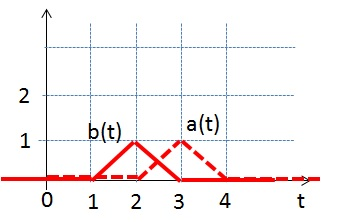
\includegraphics[scale=0.6]{images/Courbes_TD_Convolution_2_Solution_2.jpg} 
	\end{figure}
	En écrivant $a(t)=(t-2)(u(t-3)-u(t-2))+(4-t)(u(t-3)-u(t-4))$ et $b(t)=(t-1)(u(t-1)-u(t-2))+(3-t)(u(t-2)-u(t-3))$, on retrouve l'expression précédente pour y(t).
	
	\vspace{1\baselineskip}
	
	\subsubsection{Exercice 3 - Convolution de spectre}
	
	On considère deux signaux, définis par les fonctions $f_{1}(t) = cos(\omega_{1}t) et f_{2} = cos(\omega_{2}t)$. 
	
	1. Déterminez l'expression du spectre du signal $f(t)=f_{1}(t)\cdot f_{2}(t)$ (on prendra $\omega_{1} > \omega_{2}$). Représentez le graphiquement.
	
	2. Même chose avec $f_{2}(t) = sin(\omega_{2}t)$.
	
	3. Même chose avec $f_{2}(t) = sinc(t)$.
	
	4. Conclure sur l'effet de la multiplication par un signal sinusoïdal.
	
	\vspace{1\baselineskip}
	
	\textbf{\underline{Correction exercice 2}}\\
	
	1. On détermine d'abord les spectres des signaux $f_{1}$ et $f_{2}$ : $F_{1}(\omega)=\frac{\delta(\omega-\omega_{1})+\delta(\omega+\omega_{1})}{2}$ et $F_{2}(\omega)=\frac{\delta(\omega-\omega_{2})+\delta(\omega+\omega_{2})}{2}$.
	La multiplication de deux signaux dans le domaine temporel conduit à un produit de convolution de leur spectre :
	
	\begin{equation*}
	F(\omega)=F_{1}*F_{2}(\omega)=\frac{1}{4}[(\delta(\omega-\omega_{1})+\delta(\omega+\omega_{1}))*(\delta(\omega-\omega_{2})+\delta(\omega+\omega_{2})]
	\end{equation*}
	\begin{equation*}
	F(\omega)=\frac{1}{4}[\delta(\omega-\omega_{1})*\delta(\omega-\omega_{2})+\delta(\omega-\omega_{1})*\delta(\omega+\omega_{2})+\delta(\omega+\omega_{1})*\delta(\omega-\omega_{2})+\delta(\omega+\omega_{1})*\delta(\omega+\omega_{2})]
	\end{equation*}
	\begin{equation*}
	F(\omega)=\frac{1}{4}[\delta(\omega-(\omega_{1}+\omega_{2}))+\delta(\omega-(\omega_{1}-\omega_{2}))+\delta(\omega-(-\omega_{1}+\omega_{2}))+\delta(\omega-(-\omega_{1}-\omega_{2}))]
	\end{equation*}
	Dans les fréquences positives, la multiplication de ces deux signaux a conduit à deux nouvelles composantes harmoniques, de fréquences $\omega_{1}-\omega_{2}$ et $\omega_{1}+\omega_{2}$. Tout se passe comme s'il y avait eu une translation du spectre du signal $f_{1}$ d'une fréquence = $+/-\omega_{2}$ (ou inversement du spectre du signal $f_{2}$ d'une fréquence = $+/-\omega_{1}$).
	
	2. $F_{2}(\omega)=\frac{\delta(\omega-\omega_{2})-\delta(\omega+\omega_{2})}{2j}$
	
	\begin{equation*}
	F(\omega)=F_{1}*F_{2}(\omega)=\frac{1}{4j}[\delta(\omega-(\omega_{1}+\omega_{2}))-\delta(\omega-(\omega_{1}-\omega_{2}))+\delta(\omega-(-\omega_{1}+\omega_{2}))-\delta(\omega-(-\omega_{1}-\omega_{2}))]
	\end{equation*}
	
	On retrouve le même genre de spectre qu'à la question précédente, à la phase près.
	
	3. $F_{2}(\omega)=\Pi_[-1;1](\omega)$.
	
	\begin{equation*}
		F(\omega)=F_{1}*F_{2}(\omega)=\frac{1}{2}[(\delta(\omega-\omega_{1})+\delta(\omega+\omega_{1}))*\Pi_[-1;1](\omega)]
	\end{equation*}
	\begin{equation*}
	F(\omega)=\frac{1}{2}[\Pi_[-1;1](\omega-\omega_{1})+\Pi_[-1;1](\omega+\omega_{1})]
	\end{equation*}
	
	Le spectre du signal de sortie correspond de $+/-\omega_{1}$ du signal $f_{2}$.
	
	
	\vspace{1\baselineskip}
	
	
	\subsubsection{Exercice 4}
	
	On considère la fonction porte $\pi_{[-a;a]}(t)=\pi(t)$ avec $a \in \mathbb{R^{*}}$.
	
	1. Calculez le produit de convolution $s(t)=\pi(t)*\pi(t)$.
	
	2. Calculez la transformée de Fourier $\Pi(f)$ de la fonction $\pi(t)$. En déduire l'expression de la transformée de Fourier S(f) de la fonction s(t).
	
	3. Soit le signal $l(t)=\pi(t) \cdot \pi(t)$. Calculez la transformée de Fourier L(f) de la fonction l(t).
	
	On pose a = 0.5. On considère $t \in \mathbb(R)$.
	
	4. Calculez le produit de convolution $p(t)=\pi(t)*\pi(\frac{t}{2})$.
	
	5. On considère les fonctions définies par $s_{1}(t)=\pi(\frac{t-1}{2})$ et $s_{2}(t)=s_{1}(t)-s_{1}(t-2)$. Tracez $s_{1}(t)$ et $s_{2}(t)$. Calculez le produit de convolution entre $s_{1}$ et $s_{2}$.
	
	\vspace{1\baselineskip}
	
	\subsubsection{Exercice 5 - Échantillonnage}
	
	On considère le circuit de principe ci-dessous, formé d'un interrupteur idéal et appelé échantillonneur. x(t) est le signal d'entrée, h(t) le signal de commande d'ouverture/fermeture de l'interrupteur, et y(t) le signal de sortie. L'interrupteur est ouvert lorsque la commande est nulle. Il se ferme lorsque la commande h(t) = 1.
	Dans cet exercice, on considère que la commande est formée par un peigne de Dirac de période T. Dans un premier temps, le signal d'entrée est une fonction sinus cardinal (expression ..., largeur $\tau$)
	
	1. Donnez la relation entre les signaux de sortie, d'entrée et de commande.
	
	2. Tracez l'allure du signal de sortie. Le nom d'échantillonneur donné au circuit est-il justifié ? Sa présence est-il nécessaire dans les circuits de traitement de signal ?
	
	3. Donnez les transformées de Fourier des signaux x(t) et h(t) ? Esquissez leur spectre (en amplitude).
	
	4. Déterminez la transformée de Fourier du signal y(t). Esquissez son spectre dans le cas où T << $\tau$, puis dans le cas où T > $\tau$.
	
	5. Est-il possible de retrouver le signal x(t) à partir de l'acquisition du signal y(t). Comment et sous quelles conditions ?
	
	
	\newpage
	
	\chapter{Energie, puissance et corrélation}
	
	
	\subsubsection{Exercice 1}
	
	Calculez la puissance moyenne ou l'énergie totale des signaux suivants ...
	
	\subsubsection{Exercice 2}
	
	On dispose d'un spectre d'amplitude de raies après un système. Le signal est à support non borné.
	
	1. quelle est la nature du signal ? Précisez les caractéristiques du signal.
	
	2. quelle est la puissance moyenne du signal ?
	
	3. Ce signal traverse un système. On relève le spectre en amplitude en sortie de ce système (figure ci-dessous). Le système est-il linéaire ?
	
	4. Calculez la puissance moyenne du signal en sortie du système.
	
	5. On définit le taux de distorsion harmonique total (\textit{Total Harmonic Distortion} (THD) en anglais) du signal par rapport au fondamental à l'aide de l'équation suivante :
	\begin{equation*}
	THD_{F}=\frac{\sqrt{\sum_{i=2}^{+\infty}A_{i}^{2}}}{A_{1}}
	\end{equation*}
	
	 avec  $A_{i}$ l'amplitude de l'harmonique de rang i. Calculez ce taux sur les signaux d'entrée et de sortie du système.
	
	\vspace{1\baselineskip}
	
	\textbf{\underline{Correction exercice 2}}\\
	
	1. Puisqu'on ne voit qu'une seule raie à la fréquence xxx, il s'agit d'un signal (co)sinusoïdal. Comme il n'y a pas de raies visibles en f=0, le signal est centré sur 0.
	
	2. On utilise l'égalité de Parseval :
	\begin{equation*}
	P_{n}=\frac{1}{T_{0}}\int_{T_{0}}|F(n)|^{2}dt=\|F(1)|^{2}
	\end{equation*}
	
	3. L'excitation du système par le signal a créé de nouvelles composantes harmoniques. Le système est donc non linéaire.
	
	4. Egalité de Parseval :
	
	
	\subsubsection{Exercice 1}
	
	1. Soit le signal porte $x(t)=A\cdot \Pi_{\frac{b}{2}(t)}$, $b\in \mathbb{R^{*}}$.
	
		a. Calculez l'énergie totale et la puissance moyenne du signal.
		
		b. Calculez la fonction d'autocorrélation du signal.
		
		c. Calculez la densité spectrale de puissance ou d'énergie
		
		\vspace{0.5\baselineskip}
	
	2. La fonction x(t) est répétée avec une période T pour former le signal f(t). On prendra $b<\frac{T}{2}$.
	
		a. Calculez l'énergie totale et la puissance moyenne du signal.
		
		b. Calculez la fonction d'autocorrélation du signal.
		
		c. Calculez la densité spectrale de puissance ou d'énergie
	
	\vspace{1\baselineskip}
	
	\textbf{\underline{Correction exercice 1}}\\
	
	1. a. Le signal est à énergie finie : $E_{tot} = 2A^{2}b$. Sa puissance moyenne est nulle.
	
	b. Calcul de la fonction d'autocorrélation :
	\begin{equation*}
	R_{XX}(\tau)=\int_{-\infty}^{+\infty}x(t)x(t-\tau)dt
	\end{equation*}
	\begin{itemize}
		\item si $\tau < -2b$ ou $\tau > 2b$, alors $R_{XX}(\tau)=0$.
		\item si $-2b \leq \tau < 0$, alors $R_{XX}(\tau)=\int_{-b}^{\tau +b}A^{2}dt=A^{2}(\tau+2b)$.
		\item si $0 \leq \tau < 2b$, alors $R_{XX}(\tau)=\int_{\tau-b}^{ b}A^{2}dt=A^{2}(2b-\tau)$. 
	\end{itemize}
	On vérifie que la valeur de l'autocorrélation est l'origine est bien égale à l'énergie totale du signal.

	\begin{figure}[h!]
		\centering
		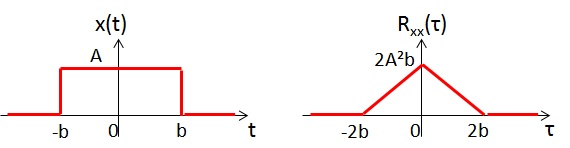
\includegraphics[scale=0.6]{images/Exo_8_1_1.jpg} 
	\end{figure}

	c. Calcul de la densité spectrale d'énergie :
	\begin{equation*}
	S_{X}(f)=\mathcal{F}[R_{XX}(\tau)]=b\cdot sinc(2bf)^{2}\cdot 2A^{2}b=2A^{2}b^{2}sinc(2bf)^{2}	
	\end{equation*}

	\vspace{0.5\baselineskip}
	
	2.a. L'énergie du signal est infinie car il est périodique. Sa puissance moyenne est égale à $\overline{P}=\frac{1}{T}\int_{-\frac{T}{2}}^{\frac{T}{2}}f(t)dt=\frac{2A^{2}b}{T}$. 

	b. La fonction d'autocorrélation est périodique, de période T. Pour chaque période, on trouve :
	\begin{itemize}
		\item pour $-\frac{T}{2}<\tau<-2b$ et $2b<\tau<\frac{T}{2}$,  $R_{FF}(\tau)=0$.
		\item pour $-2b \leq \tau < 0$, alors $R_{YY}(\tau)=\frac{A^{2}(\tau+2b)}{T}$.
		\item si $0 \leq \tau < 2b$, alors $R_{XX}(\tau)\frac{A^{2}(2b-\tau)}{T}$. 
	\end{itemize}
	On vérifie que la valeur de l'autocorrélation est l'origine est bien égale à la puissance moyenne du signal.
	
	\vspace{0.5\baselineskip}
	
	c. La densité spectrale de puissance est donnée par la transformée de Fourier de la fonction d'autocorrélation. Celle-ci étant périodique (fréquence $f_{0}=\frac{1}{T})$, on trouve :
	\begin{equation*}
	S_{F}(f)=\mathcal{F}[R_{FF}(\tau)]=\frac{2A^{2}b^{2}}{T}\sum_{n=-\infty}^{+\infty}sinc(2bnf_{0})\delta(f(-nf_{0}))
	\end{equation*}
	
	
	\vspace{1\baselineskip}	
	
	\subsubsection{Exercice 2}
	
	Un signal noté $x(t)=cos(2\pi f_{0}t)$ excite un filtre passe-bas d'ordre 1, dont la fréquence de coupure est $f_{0}$. Le signal en sortie du filtre est noté y(t).
	
	\vspace{0.5\baselineskip}	
	
	1. Donnez l'expression de la transformée de Fourier X(f) du signal x(t). Tracez son module et son argument.
	
	\vspace{0.5\baselineskip}
	
	2. Donnez l'expression de la fonction de transfert H(f) du filtre. Tracez son module et son argument dans le diagramme de Bode. Quel est son gain et son déphasage en $f_{0}$ ?
	
	\vspace{0.5\baselineskip}
	
	3. A partir de X(f) et H(f), déterminez la transformée de Fourier Y(f) du signal y(t).
	
	\vspace{0.5\baselineskip}
	
	4. Déterminez l'expression du signal y(t) à partir de Y(f).
	
	\vspace{0.5\baselineskip}
	
	5. Calculez la puissance moyenne du signal d'entrée. En déduire celle du signal de sortie.
	
	\vspace{1\baselineskip}	
	
	\subsubsection{Correction exercice 2}
	
	1. $X(f)=\frac{1}{2}(\delta(f-f_{0})+\delta(f+f_{0}))$
	
	
	2. $H(f)$$\frac{1}{1+j\frac{f}{f_{0}}}$. Par convention, le module et la phase sont tracés uniquement pour les fréquences positives dans le diagramme de Bode. Il est intéressant de les tracer aussi pour les fréquences négatives, pour la suite de l'exercice.
	
	En $f= f_{0}$, on a $|H(f_{0})|=\frac{1}{\sqrt{2}}$ et $Arg(H(f_{0}))=-\frac{\pi}{4}$.
	
	3. \begin{equation*}
	Y(f)=H(f)X(f)=\frac{1}{2}(H(f_{0})\delta(f-f_{0})+H(-f_{0})\delta(f+f_{0}))
	\end{equation*}
	\begin{equation*}
	Y(f)=\frac{1}{2}(\frac{1}{1-j}\delta(f-f_{0})+\frac{1}{1+j}\delta(f+f_{0}))
	\end{equation*}
	\begin{equation*}
	Y(f)=\frac{1}{2\sqrt{2}}(e^{-j\frac{\pi}{4}}\delta(f-f_{0})+e^{j\frac{\pi}{4}}\delta(f+f_{0}))
	\end{equation*}

	
	4. On détermine l'expression de y(t) à partir de la transformée de Fourier inverse de Y(f):
	
	\begin{equation*}
	y(t)=\mathcal{F}^{-1}[Y(f)]=\int_{-\infty}^{+\infty}\frac{1}{2\sqrt{2}}(e^{-j\frac{\pi}{4}}\delta(f-f_{0})+e^{j\frac{\pi}{4}}\delta(f+f_{0}))e^{j2\pi ft}df
	\end{equation*}
	
	En utilisant la propriété d'échantillonnage de l'impulsion de Dirac :
	\begin{equation*}
	y(t)=\frac{1}{2\sqrt{2}}(e^{j(2\pi f_{0}t-\frac{\pi}{4})}+(e^{-j(2\pi f_{0}t-\frac{\pi}{4})})
	\end{equation*}
	\begin{equation*}
	y(t)=\frac{1}{\sqrt{2}}cos(2\pi f_{0}t-\frac{\pi}{4})
	\end{equation*}
	
	Le filtre atténue bien le signal d'un facteur $\frac{1}{\sqrt{2}}$ et introduit un déphasage négatif de $-\frac{\pi}{4}$.
	
	\vspace{0.5\baselineskip}	
	
	5. On peut calculer la puissance moyenne $\overline{P_{X}}$ du signal d'entrée à partir de sa densité spectrale de puissance :
	\begin{equation*}
	S_{X}(f)=|X(f)|^{2}
	\end{equation*}
	\begin{equation*}
	\overline{P_{X}}=\int_{-\infty}^{+\infty}S_{X}(f)df=\int_{-\infty}^{+\infty}\frac{1}{4}|\delta(f-f_{0})+\delta(f+f_{0})|^{2}df
	\end{equation*}
	\begin{equation*}
	\overline{P_{X}}=\int_{-\infty}^{+\infty}\frac{1}{4}(\delta(f-f_{0})+\delta(f+f_{0}))df=\frac{1}{2}
	\end{equation*}
	On peut confirmer ce résultat en intégrant le signal temporel sur une période.
	
	On peut calculer la puissance moyenne du signal de sortie à partir de sa densité spectrale de puissance :
	\begin{equation*}
	S_{Y}(f)=|Y(f)|^{2}=|H(f)|^{2}S_{X}(f)
	\end{equation*}
	\begin{equation*}
	\overline{P_{Y}}=\int_{-\infty}^{+\infty}S_{Y}(f)df=\int_{-\infty}^{+\infty}\frac{1}{4}|H(f)|^{2}|\delta(f-f_{0})+\delta(f+f_{0})|^{2}df
	\end{equation*}
	\begin{equation*}
	\overline{P_{Y}}=\frac{1}{4}\int_{-\infty}^{+\infty}|H(f)|^{2}(\delta(f-f_{0})+\delta(f+f_{0}))df=\frac{1}{4}(|H(f_{0})|^{2}+|H(-f_{0})|^{2})
	\end{equation*}
	Le filtre étant réel, on a $|H(f_{0})|=|H(-f_{0})|$, donc on trouve : 
	\begin{equation*}
	\overline{P_{Y}}=\frac{1}{4}2|H(f_{0})|^{2}=\frac{1}{2}(\frac{1}{\sqrt{2}})^{2}=\frac{1}{4}
	\end{equation*}
	Le filtre atténuant l'amplitude d'entrée d'un facteur $\frac{1}{\sqrt{2}}$, la puissance du signal de sortie est donc divisée par 2.
	
	
	
		


	
	
	
	
	\vspace{1\baselineskip}	
	
	
	
	
\end{document}